\section{Control Unit}

The control unit interprets instructions (opcodes) from the Instruction Memory and decodes them to determine what operations are to be performed. In the following subsections, we will discuss the Control Unit's behavior and how it is implemented.

\subsection{Behavior of Control Unit}

\begin{figure}[H]
    \centering
    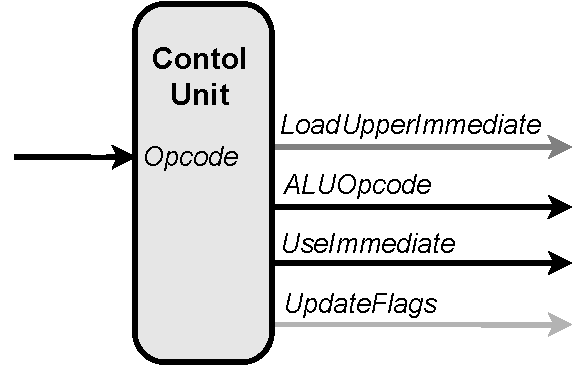
\includegraphics[width=.5\columnwidth]{pics/diagrams/riscv/modules/control_unit}
    \caption{Interface of the Control Unit}
    \label{fig:control_unit_module}
\end{figure}

When receiving an \codeword{Opcode}, the Control Unit outputs four different signals:
\begin{itemize}
    \setlength\itemsep{3pt}
    \item \codeword{LoadUpperImmediate}, which tells whether we need to store data from ALU or instruction (to execute LUI instruction);
    \item \codeword{ALUOpcode}, which sends ALU 0 or 1 depending on the type of operation we are performing (multiplication, division);
    \item \codeword{UseImmediate}, which tells whether the C operand is an immediate value or the value from the register file;
    \item \codeword{UpdateFlags}, which indicates whether the Register File should update flags after the operation or not.
\end{itemize}
    
An overview of the input and output signals of the Control Unit is shown in Figure \ref{fig:control_unit_module}.


\subsection{Implementation of Control Unit}

We have five different opcodes to be handled; they are 3 bits long and stored in [15:13] bits of the instruction. In the following, we will discuss the behavior of the Control Unit for each of these opcodes.


\textbf{Load Upper Immediate (LUI, 011)}

The dummy signal is sent to all inputs of ALU because there is no computation to do.

\begin{itemize}
    \setlength\itemsep{2pt}
    \item \codeword{ALUOpcode} = 0 (dummy signal);
    \item \codeword{UseImmediate} = 0 (dummy signal);
    \item \codeword{LoadUpperImmediate} = 1 -- in this case, we ignore ALU output and take the immediate value from the instruction;
    \item \codeword{UpdateFlags} = 0 -- there is no flags to update.
\end{itemize}

In all the following cases, the upper immediate value is ignored; thus, \codeword{LoadUpperImmediate} is set to 0.

\textbf{Multiplication (MUL, 111)}
\begin{itemize}
    \setlength\itemsep{2pt}
    \item \codeword{ALUOpcode} = 1 (multiplication);
    \item \codeword{UseImmediate} = 0 (RRR operation);
    \item \codeword{LoadUpperImmediate} = 0;
    \item \codeword{UpdateFlags} = 1 -- to renew the flags' state.
\end{itemize}

\textbf{Multiplication Immediate (MULi, 001)}
\begin{itemize}
    \setlength\itemsep{2pt}
    \item \codeword{ALUOpcode} = 1 (multiplication);
    \item \codeword{UseImmediate} = 1 (RRi operation);
    \item \codeword{LoadUpperImmediate} = 0;
    \item \codeword{UpdateFlags} = 1 -- to renew the flags' state.
\end{itemize}

\textbf{Division (DIV, 000)}
\begin{itemize}
    \setlength\itemsep{2pt}
    \item \codeword{ALUOpcode} = 0 (division);
    \item \codeword{UseImmediate} = 0 (RRR operation);
    \item \codeword{LoadUpperImmediate} = 0;
    \item \codeword{UpdateFlags} = 1 -- to renew the flags' state.
\end{itemize}
    
\textbf{Division Immediate (DIVi, 010)}
\begin{itemize}
    \setlength\itemsep{2pt}
    \item \codeword{ALUOpcode} = 0 (division);
    \item \codeword{UseImmediate} = 1 (RRi operation);
    \item \codeword{LoadUpperImmediate} = 0;
    \item \codeword{UpdateFlags} = 1 -- to renew the flags' state.
\end{itemize}

In the code, this logic is implemented using the case keyword:
\begin{code}[12]{Opcode switch-statement example}
    always @(Opcode) begin
	case (Opcode)
        // MUL
        3'b111: begin
            ALUOpcode = 1;
            UseImmediate = 0;
            LoadUpperImmediate = 0;
            UpdateFlags = 1;
        end
    ...
\end{code}
